\bigskip
\section{Notación de nudos.}
Ya sabemos qué son los nudos y algunas nociones esenciales sobre los mismos, pero aún no sabemos asociar una notación concreta a un nudo. En esta sección vamos a ver algunas de las notaciones más comunes de los nudos. 

\begin{center}
	\item \subsection{Notación de Dowker:}
\end{center}
Se trata de una notación muy sencilla para describir la proyección de un nudo. La notación en sí es una secuencia de números enteros, veamos cómo se obtiene:\\

Consideramos una orientación en la proyección de n cruces y asignamos el valor 1 al primer cruce que nos encontremos. Continuamos por la proyección y asignamos el valor 2 al siguiente cruce. Vamos repitiendo el proceso hasta pasar por cada cruce un par de veces (una vez por el undercrossing y otra por el overcrossing). Como resultado tendremos un número par y un número impar por cada cruce de la proyección. \\

Finalmente es necesario asignar los signos a cada uno de estos $2n$ números. Los números pares que correspondan a un overcrossing tendrán signo negativo. Veamos un ejemplo con el nudo trébol que podemos ver en la figura \ref{dow1}:\\
   \begin{figure}[h!]
   	\centering
   	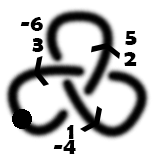
\includegraphics[width=4cm]{inudos/3fcon2dow.png}
   	\caption{Numeración de cruces-Dowker.}
   	\label{dow1} 
   \end{figure}
   
  Tendríamos los pares (1,-4), (3,-6) y (5,2). La notación de Dowker sería -4 -6 2 pues nos quedamos únicamente con los números pares en el orden que indican los números impares.\\

\begin{center}
	\item \subsection{Notación de Gauss:}
\end{center}
La notación de Gauss es una notación parecida a la de Dowker. Consideremos de nuevo una orientación en la proyección de n cruces de un nudo.\\

En este caso cada vez que pasamos por un cruce, tendremos un solo número asignado. De este modo la secuencia de números de la notación se compone de $2n$ elementos con valores desde 1 hasta n, cada uno de ellos repetido dos veces.\\

Consideramos una orientación en la proyección de n cruces y asignamos el valor 1 al primer cruce que nos encontremos. Realizamos el siguiente proceso: continuamos por la proyección hasta el siguiente cruce. Si ya hemos pasado por él, anotamos el número de cruce que tenga asociado. Si no hemos pasado anteriormente por él, asignamos el siguiente número de cruce.\\

Finalmente es necesario asignar los signos a cada uno de esos $2n$ números. Los números que representen uncrossings tendrán signo negativo. Veamos la notación de Gauss para el nudo trébol.\\
   \begin{figure}[h!]
   	\centering
   	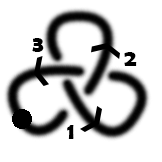
\includegraphics[width=4cm]{inudos/3fcon2gaus.png}
   	\caption{Numeración de cruces-Gauss.}
   	\label{gaus1} 
   \end{figure} 
Si vamos haciendo el recorrido partiendo desde el punto grueso indicado tendríamos la secuencia de números: -1 2 -3 1 -2 3. Esta sería su notación de Gauss.

\begin{center}
	\item \subsection{Notación de Conway:}
\end{center}
Por último vamos a ver una notación que puede resultar algo más compleja pero que tiene gran uso e interés, sobre todo en la tería del ADN. \\

\underline{\textbf{Definición:}}\\
Un \textbf{enredo} o tangle de una proyección de un enlace es una región de la proyección rodeada por una bola de modo que las dos cuerdas enlazadas de la proyección tocan la bola exactamente en cuatro puntos. A estos puntos los denotaremos como NO, NE, SO y SE.\\

En la figura \ref{conw1} vemos un enredo general y un ejemplo particular de un enredo.\\
   \begin{figure}[h!]
   	\centering
   	\subfigure[Enredo general]{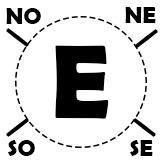
\includegraphics[width=4.5cm]{inudos/en1.png}}
   	\subfigure[Ejemplo de enredo]{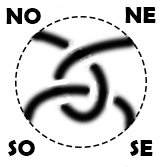
\includegraphics[width=4.5cm]{inudos/en2.png}}
   	\caption{Enredos}
   	\label{conw1} 
   \end{figure} 

Pero la idea es trabajar con enredos más sencillos como son los que vemos en la figura \ref{conw2}. La notación se corresponde con el número de cruces que tiene el enredo con signo positivo y negativo según se ve en las imágenes.\\
   \begin{figure}[h!]
   	\centering
   	\subfigure[Enredo $\infty$]{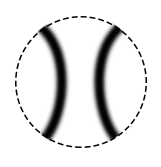
\includegraphics[width=3cm]{inudos/en3.png}}
   	\subfigure[Enredo 0]{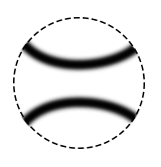
\includegraphics[width=3cm]{inudos/3enrot.png}}
   	
   	\subfigure[Enredo 4]{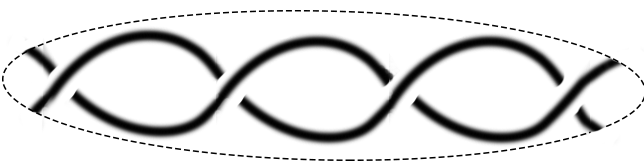
\includegraphics[width=8cm]{inudos/en4.png}}
   	
   	\subfigure[Enredo -4]{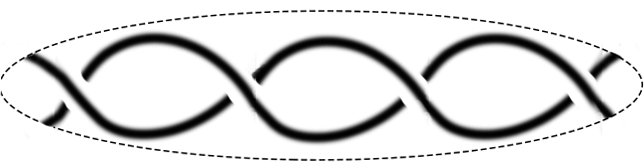
\includegraphics[width=8cm]{inudos/en4conneg.png}}
   	\caption{Tipos básicos de enredos.}
   	\label{conw2} 
   \end{figure} 

Haciendo uso de estos enredos básicos podemos construir nuevos enredos uniendo, respectivamente, los extremos NE y SE de un enredo con los extremos NO y SO del otro enredo. A esta operación se le conoce como suma de enredos.\\
Además, disponemos de una operación de multiplicación: reflejaremos el primer enredo y hacemos la operación de suma.\\
A los enredos construidos con estas operaciones se les conoce con \textbf{enredos racionales}. Podemos ver un esquema básico estas dos operaciones en la imagen \ref{conw3}:\\
   \begin{figure}[h!]
   	\centering
   	\subfigure[Operacion suma]{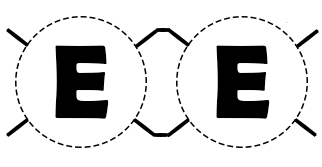
\includegraphics[width=8cm]{inudos/ensum.png}}
   	\subfigure[Operacion multiplicacion]{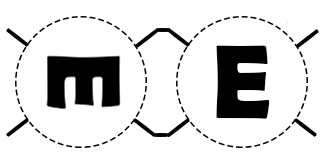
\includegraphics[width=8cm]{inudos/enmul.png}}
   	\caption{Operaciones con enredos.}
   	\label{conw3} 
   \end{figure}

En la figura \ref{conw4} podemos ver un ejemplo de un enlace más complejo:
\begin{figure}[h!]
	\centering
	
\includegraphics[width=4cm]{inudos/en5fin.png}
	\caption{Enlace -2 3 2}
	\label{conw4} 
\end{figure}

A partir de estos enredos podemos construir proyecciones de nudos enlazando los puntos NO con NE y los puntos SO con SE. La notación del nudo corresponde con la notación que le damos a su enredo.\\ 

Nos interesa ver si dos proyecciones de nudos representan al mismo nudo, luego nos interesa ver si dos enredos son equivalentes. Veamos qué quiere decir que sean equivalentes:\\

\underline{\textbf{Definición:}}\\
Diremos que dos enredos son equivalentes si podemos pasar de un enredo al otro mediante los movimientos de Reidemeister, que vimos en la sección \ref{seccion4}, manteniendo los cuatro extremos fijos en la bola imaginaria. \\

Ver si dos enredos son equivalentes por definición no es viable de modo que vamos a aplicar otro método: consiste en calcular la fracción continua asociada a cada enredo.\\

\underline{\textbf{Definición:}}\\
Sea un enredo con notación $a_{n}...a_{1}a_{0}$. Su\textbf{ fracción continua} es una expresión del tipo:
\begin{equation}
    a_{0} + \frac{1}{a_{1} + \frac{1}{a_{2} + \frac{1}{...a_{n}}}}
\end{equation}
siendo $a_{i} \in \mathds{Z},  \forall i = 0,1,..,n.$\\

\begin{teo}
Dos enredos racionales son equivalentes si y solo si sus fracciones continuas toman el mismo valor. 
\end{teo}

Veamos un ejemplo. Consideramos los enredos racionales -2 3 2 y 3 -2 3 que vemos en la figura \ref{conw5}.\\
\begin{figure}[h!]
	\centering
	\subfigure[Enlace -2 3 2]{
\includegraphics[width=4cm]{inudos/en5fin.png}}
	\space
	\subfigure[Enlace 3 -2 3]{
\includegraphics[width=4cm]{inudos/en6fin.png}}
	\caption{Enlaces equivalentes}
	\label{conw5} 
\end{figure}

A simple vista resulta difícil confirmar que sean equivalentes. Vamos a obtener sus fracciones continuas asociadas:\\
$-2 \hspace{1cm} 3 \hspace{1cm} 2 \hspace{1cm}$ tiene fracción continua
\begin{equation}
 2 + \frac{1}{3 + \frac{1}{-2}} = \frac{12}{5}
\end{equation}

$3 \hspace{1cm} -2 \hspace{1cm} 3 \hspace{1cm}$ tiene fracción continua
\begin{equation}
3 + \frac{1}{-2 + \frac{1}{3}} = \frac{12}{5}
\end{equation}
Ambas fracciones continuas son iguales, luego los enredos -2 3 2 y 3 -2 3 son equivalentes. 
